

\subsection{Locality-aware  overlay network \label{ssec:lao}}

We here present our lazy locality-aware overlay network which underlies the VM
scheduling platform we developed. It is made of two layers. The lower layer is
mainly an implementation of the Vivaldi protocol (whose core mechanisms were
described earlier) making nodes (that are initially interconnected arbitrarily)
aware of their position in the platform. 

Based on these coordinates, the higher layer is responsible for building
dynamically an locality-aware overlay. This layer takes its roots in the classic
Dijkstra's shortest path algorithm to collect a set of close nodes starting from
a given position.

%%\subsubsection*{Giving a position to nodes}



% \AL[CT/MB]{C'est pas de la redite d'avant tout ce paragraphe, je veux dire ca
%   devrait pas etre plutot dans background non ?}

% \MB[AL]{Non, dans le sens ou on est plus descriptifs. Dans le paragraphe
%   precedent, on voit plutot Vivaldi comme une boite noire (sa fonctionalite).}

% As already mentioned, Vivaldi~\cite{dabek:2001:sigcomm04} is a
% distributed protocol assigning coordinates in the plane to nodes of a
% distributed set of nodes. Each node is equipped with a \emph{view} of the
% network, \emph{i.e.}, a set of nodes it knows. Coordinates obtained by a node
% reflects its \emph{position} in the network, \emph{i.e.}, close nodes in the
% network are given close coordinates in the plane. To achieve this, each node
% checks the round trip time between itself and another node (randomly chosen
% among nodes in its view) and adapts its distance (by changing its coordinates)
% with this node in the plane accordingly. % See Figure~\ref{fig:vivaldi_before} and
% % Figure~\ref{fig:vivaldi_after} for an illustration of 4 nodes~(A, B, C and D)
% % moving according to the Vivaldi protocol.
% A globally accurate positioning of nodes can be
% obtained if nodes have a few long-distance nodes in their
% view. Note that these long distance links can be easily
% maintained.

% \begin{figure}[!b]
% 	\vspace*{-.3cm}
%   \begin{minipage}[c]{.45\linewidth}
%    \hspace*{-0.5cm}
%       	\centering 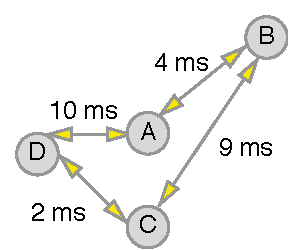
\includegraphics[width=3.4cm]{./FIGS/vivaldi_before.pdf}

%    \hspace*{0.5cm}
% 		\caption{Vivaldi plot before updating positions. Each node pings other nodes. Each node maintains a map of distance.}
% \label{fig:vivaldi_before}
%    \end{minipage}
% \hspace*{0.6cm}
%    \begin{minipage}[c]{.45\linewidth}
%    	\centering 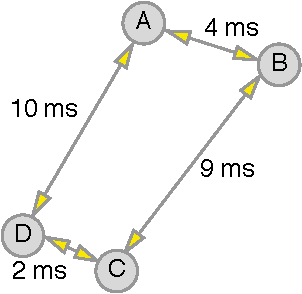
\includegraphics[width=3.4cm]{./FIGS/vivaldi_after.pdf}
% 		\caption{Vivaldi plot after updating positions. The computed
%                   positions of other nodes have been updated.}
% 		\label{fig:vivaldi_after} 
%   \end{minipage} \hfill
% \end{figure}

\subsubsection*{Searching for Close Nodes}

Once the map of Vivaldi is achieved (each node knows its coordinates), we are
able to decide whether two nodes are \emph{close} by calculating their
distance. However, the view of each node does not \emph{a priori} contain its
closest nodes. Therefore, we need additional mechanisms to locate a set of nodes
that are close to a given initial node -- Vivaldi gives a \emph{location} to
each node, not a neighborhood. We use a modified distributed version of the
classic Dijkstra's shortest path algorithm. The goal is to build a
\emph{spiral}\footnote{The term \emph{spiral} is here a misuse of language,
since the graph actually drawn in the plane might contain crossing edges.}
interconnecting the nodes in the plane that are the closest ones to a given
initial node.

Let us consider that our initial point is a node called $I$. The first step is
to find a node to build a two-node spiral with $I$. Such a node is sought in the
view of $I$ by selecting the node, say $S$, having the smallest distance with
$I$. $I$ then sends its view to $S$, $I$ stores $S$ as its successor in the
spiral, and $S$ adds $I$ as its predecessor in the spiral. Then $I$ forwards its
view to $S$. $S$ creates a new view by keeping the $n$ nodes which are the
closest to $I$ in the views of $I$ and $S$. This last view is then referred to
as the \emph{spiral view} and is intended to contain a set of nodes among which
to find the next step of the spiral. Then $S$ restarts the same process: among
the spiral view, it chooses the node with the smallest distance to $I$, say
$S'$, and adds it in the spiral -- $S$ becomes the predecessor of $S'$ and $S'$
becomes the successor of $S$. Then, the spiral view is sent to $S'$ which
updates it with the nodes it has in its own view. The process is repeated until
enough nodes have been gathered (which is a parameter sent by the application).

Note that one risk is to be blocked by having a spiral view containing only
nodes that are already in the spiral, leading to the impossibility to build the
spiral further. However, this problem can be easily addressed by forcing the
presence of a few long distance nodes whenever it is updated.


\subsubsection*{Learning}

Applying the protocol described above, the quality of the spiral is
questionable in the sense that the nodes that are actually close to the initial
node $I$ may not be included.%  The only property ensured is that one step
% forward on the built path always takes us further from the initial node.
%
To improve the \emph{quality} of the spiral, \emph{i.e.}, reduce the average
distance between the nodes it comprises and the initial node, we rely on a
learning mechanism coming with no extra communication cost: when a node is
contacted for becoming the next node in one spiral, and receives the associated
spiral view, it can also keep the nodes that are the closest to itself, thus
potentially increasing the quality of a future spiral construction. Such an
improvement through learning is illustrated in Figure~\ref{fig:learning}.


\begin{figure}[ht]
  {
    \begin{center}{
	\begin{minipage}{.3\linewidth}
	  \begin{center}
	    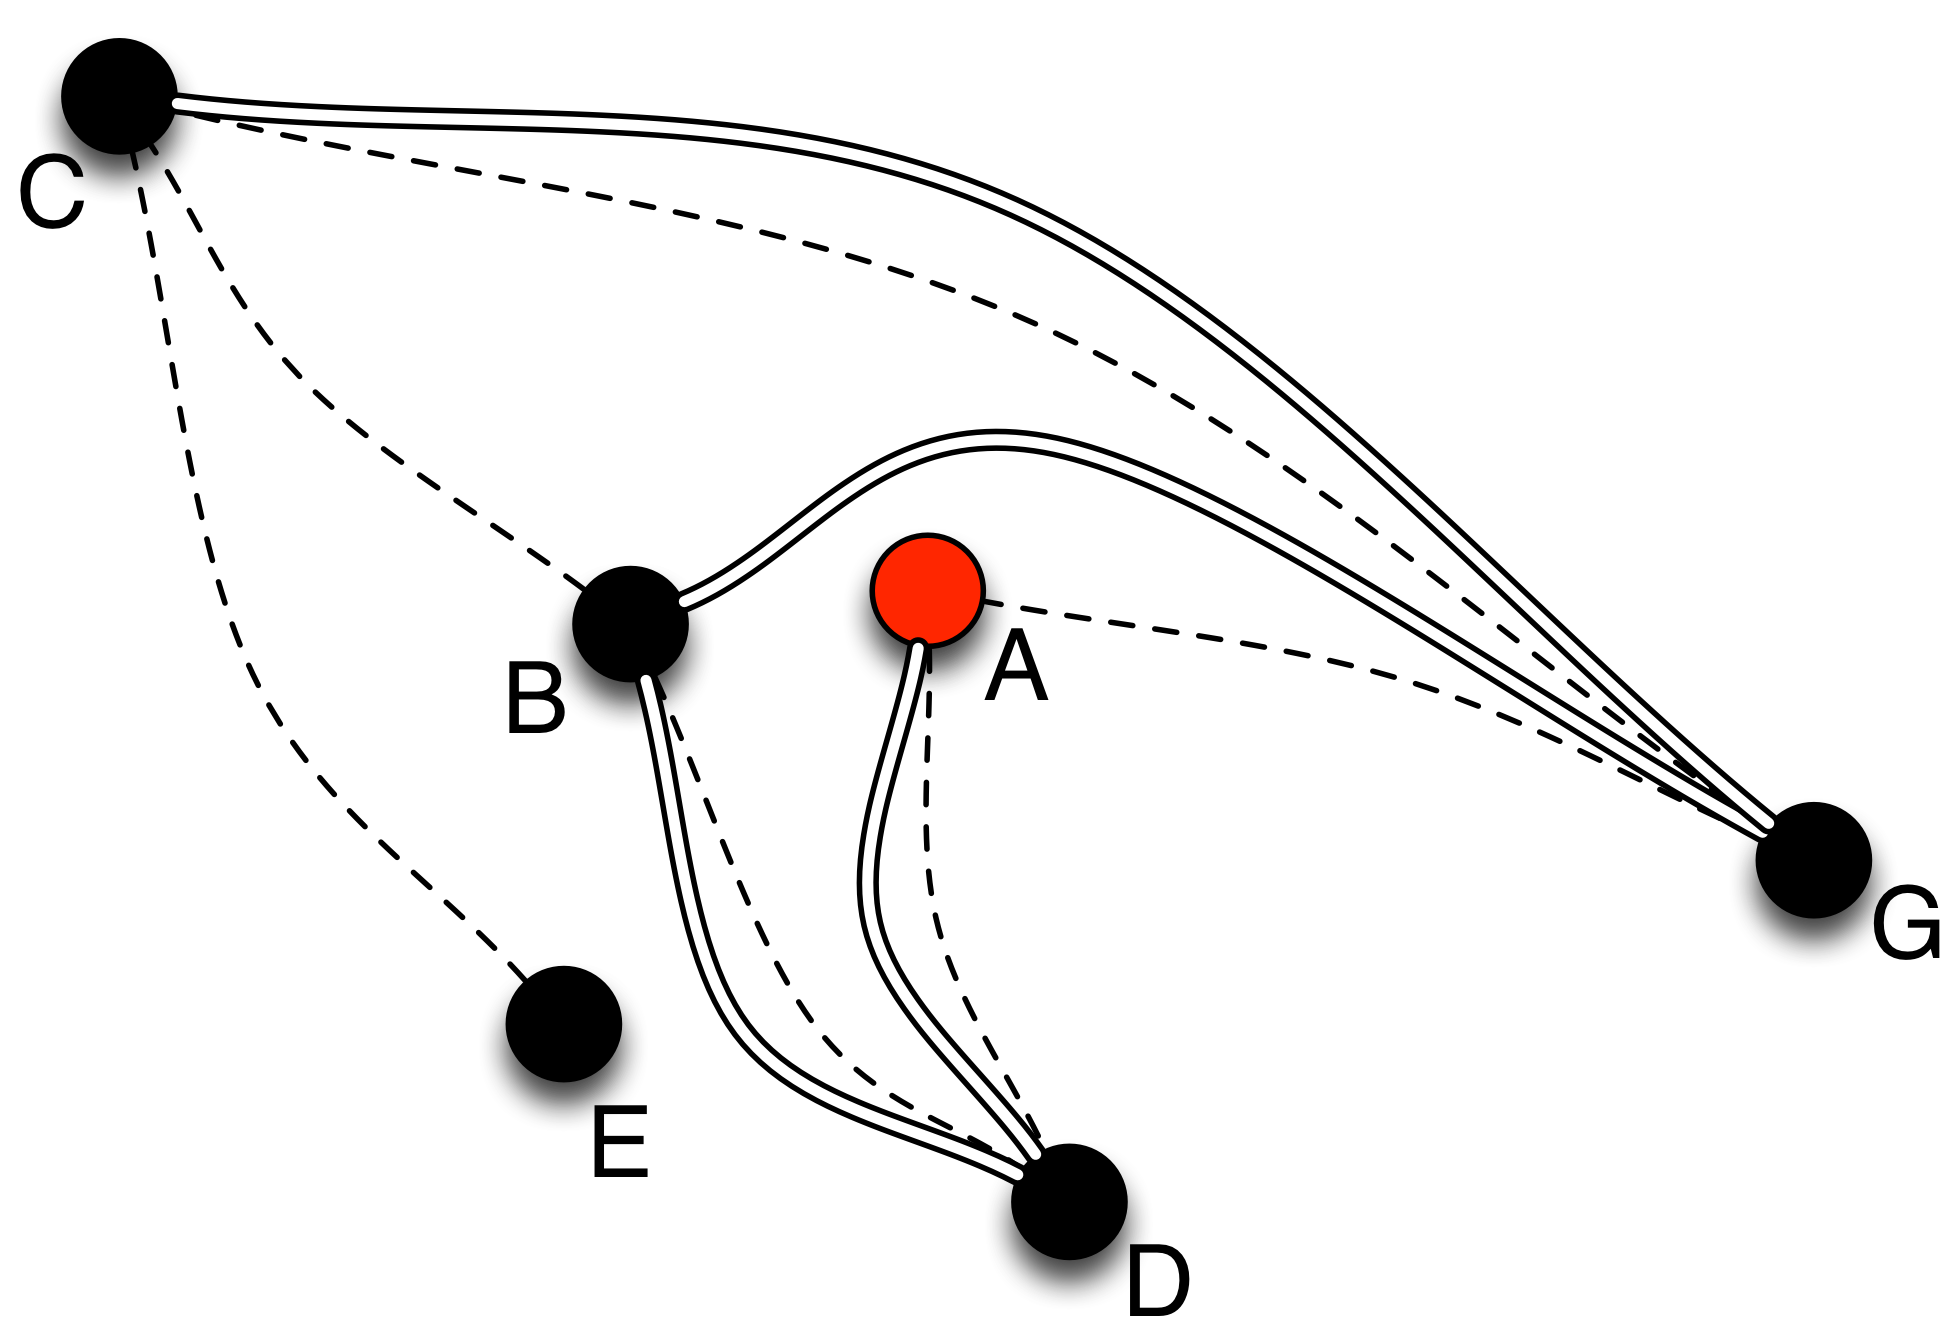
\includegraphics[width=1.05\linewidth]{Figures/learning1.png}\\(a)
	  \end{center}
	\end{minipage}
	~
	\begin{minipage}{.3\linewidth}
	  \begin{center}
	    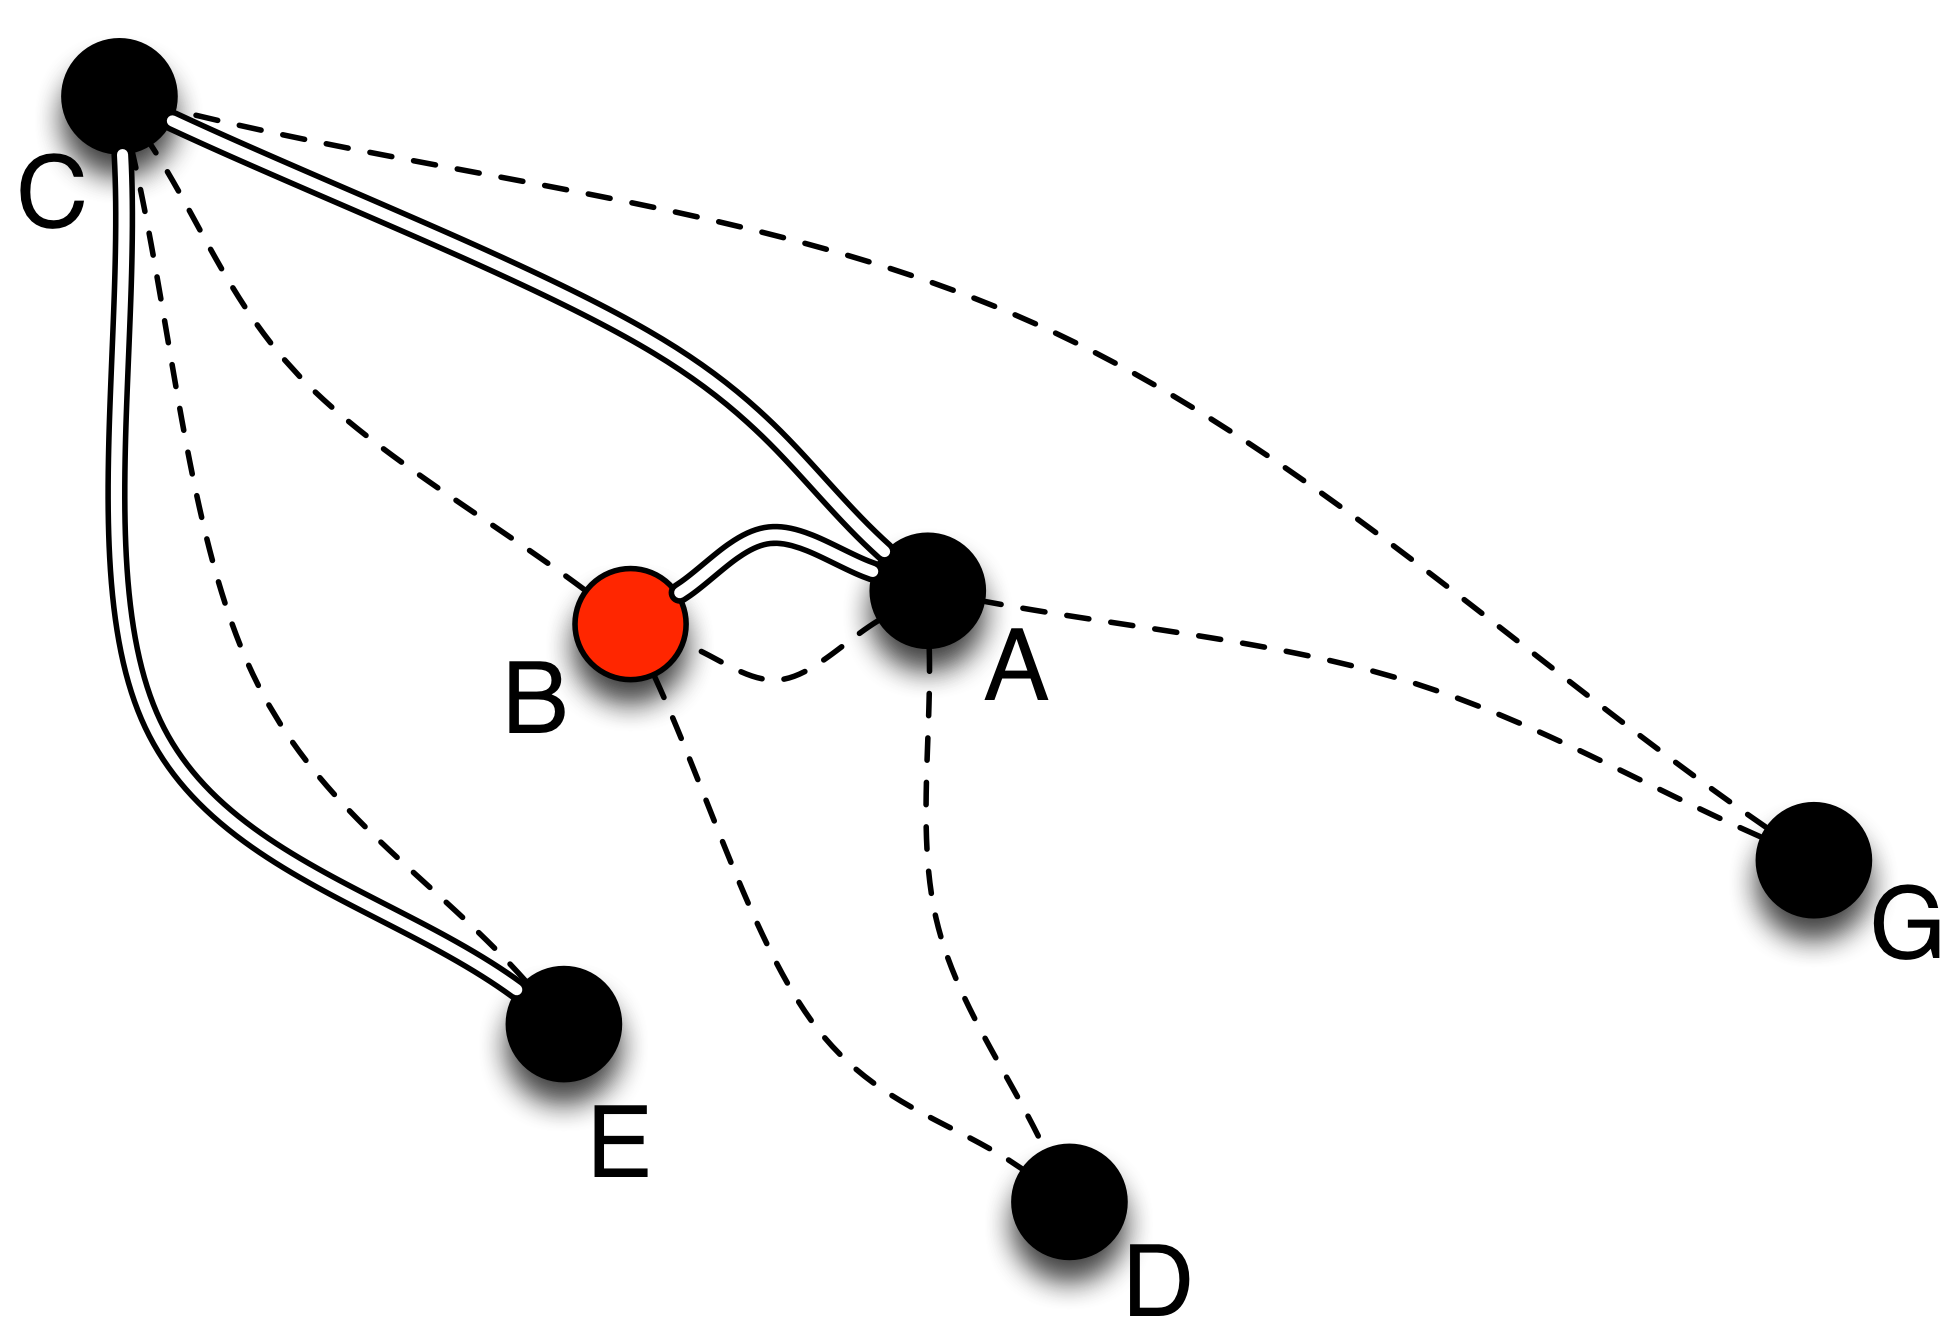
\includegraphics[width=1.05\linewidth]{Figures/learning2.png}\\(b)
	  \end{center}
	\end{minipage}
        ~
	\begin{minipage}{.3\linewidth}
	  \begin{center}
	    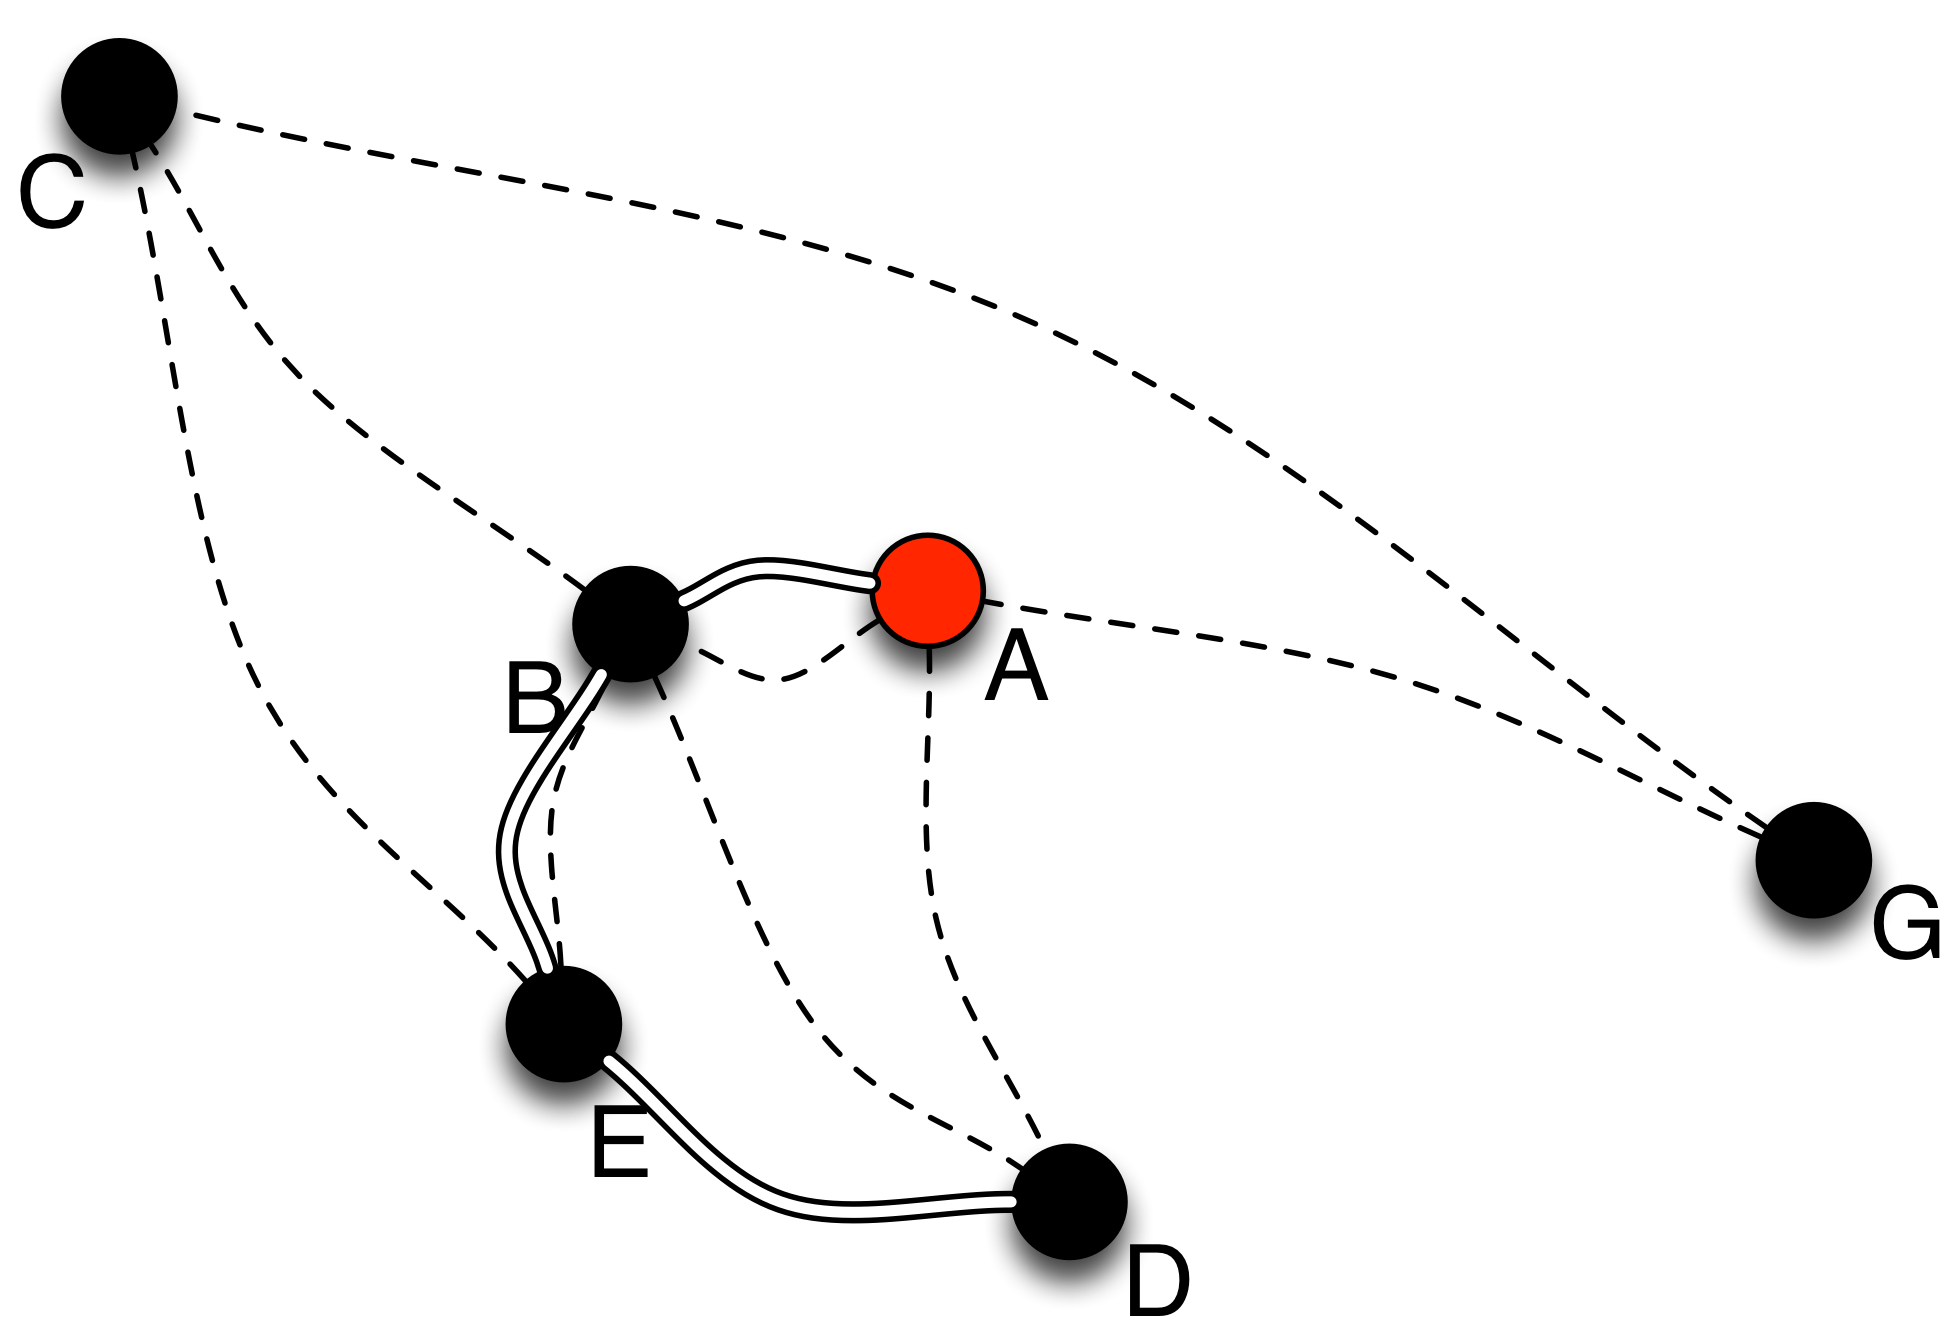
\includegraphics[width=1.05\linewidth]{Figures/learning3.png}\\(c)
	  \end{center}
	\end{minipage}
	\caption{Learning mechanism: (a) the initial view of each node are
          materialized by the dashed lines. Given these views, the spiral
          obtained from node A is represented by the double thick lines. In
          particular, this spiral allowed $A$ and $B$ to discover each
          others. (b) If $B$ starts building a spiral, it will start by
          contacting $A$. 

\label{fig:learning}} }
      \end{center}
}
\end{figure}

\AL[CT/MB]{Est ce qu'un schema n'aurait pas du sens ici ? si possible en se
  reappuyant sur le schema precedent avec les 3 clusters ? }

\MB[AL]{?a risque de prendre pas mal de place. Mais pourquoi pas. figure +
  explication de la figure... Notre id?e est de mettre plusieurs figures ... Au
  moins 3 pour illustrer un scenario d'am?lioration d'une spirale sortant d'un
  noeud donne. On essaye de faire ?a ce soir. On pr?cise que si ensuite tu
  decides de l'enlever tu nous devras 1 million de dollars.}

\subsection{PeerActor: A Building Block to Abstract Overlays}
%
%%   * Construire des algos distribues fonctionnant en reseau est dur: couts 
%% 	  impliques par la tolerance aux pannes et synchro.
%%   * Ces couts sont parfois dus aux modeles de programmation.
%Building a distributed algorithm that works at large scale is complex: fault
%tolerance, synchronization and network overhead can have a cost that 
%significantly impact on performance and scalability. This can be the result of a
%bad software design, or the consequence of the use of an inapropriate 
%programming model for a given situation, as sharing states in a distributed
%context.
%
%%   * La collaboration entre processus peut se faire de deux maniere:
%%       A) partage d'etat.
%%       B) echange de message.
%This is especially true in situation where a process share a ressource with some 
%other processes. This situation, also known as \emph{race condition situation}, 
%has been thoroughly studied, which led to different ways to organize 
%collaboration between concurrent actors that have to work concurrently:
%
%\begin{description}
%
%	\item [Shared state] : A ressource is shared between different processes: it
%	requires that each process waits for its turn before acquiring it for use.
%	This property can be guaranteed by using locks to control acces to shared
%	ressource : processes have to wait that the ressource becomes free
%	before using it.
%
%	\item [Message passing] : Each process has its own state and collaborate
%	with other processes by exchange of messages. In the case of the actor model 
%	\cite{Hewitt1973}, a process becomes an \emph{actor} wich processes one
%	message at a time. This is a lock free approach with no	shared state.
%
%\end{description}
%
%%   * les verrous sont des nids a deadlocks.
%% 	* DVMS utilise le modele d'acteurs:
%%		- chaque instance ne communique qu'avec des messages.
%%		- on favorise les collaborations proches.
%Locking ressources often leads to deadlock \cite{agha:1986}, which can have
%a significant impact on performance and scalability. That is why we decided to
%leverage the actor model to reoarganize DVMS: each instance will collaborate
%by exclusively exchanging messages and priority will be given to collabarotion
%between close instances.
%
%%   * ainsi on a créé une librarie qui:
%%		- favorise le dvlpt d'appli distribuée.
%%		- se base sur des langages/frameworks modernes.
%%	* la librairie se base sur la prog fonctionnelle et le peerActor.
%With that in mind, we created a new library whose role is to ease the

The DVMS proposal can be divided in two major
components: on the one hand the ring overlay and on the other hand, the
protocol in charge of detecting and resolving scheduling issues.  As our goal
consists in taking into account locality criteria without changing the protocol
of DVMS, we designed a building block, \ie \emph{the Peer actor}, that enabled
us to revisit DVMS by abstracting the overlays it relies on.  At
coarse-grained, the Peer actor can be seen as a generic layer for high level
distributes services, providing network abstractions and robust communication
between agents deployed on each node.  By leveraging the Peer actor API,
developers can focus on the service itself without dealing with node
apparitions/removals and network disconnections. 

%\begin{figure}[h!]
\begin{wrapfigure}{r}{0.3\linewidth}
\vspace{-.7cm}\hspace*{.2cm}
  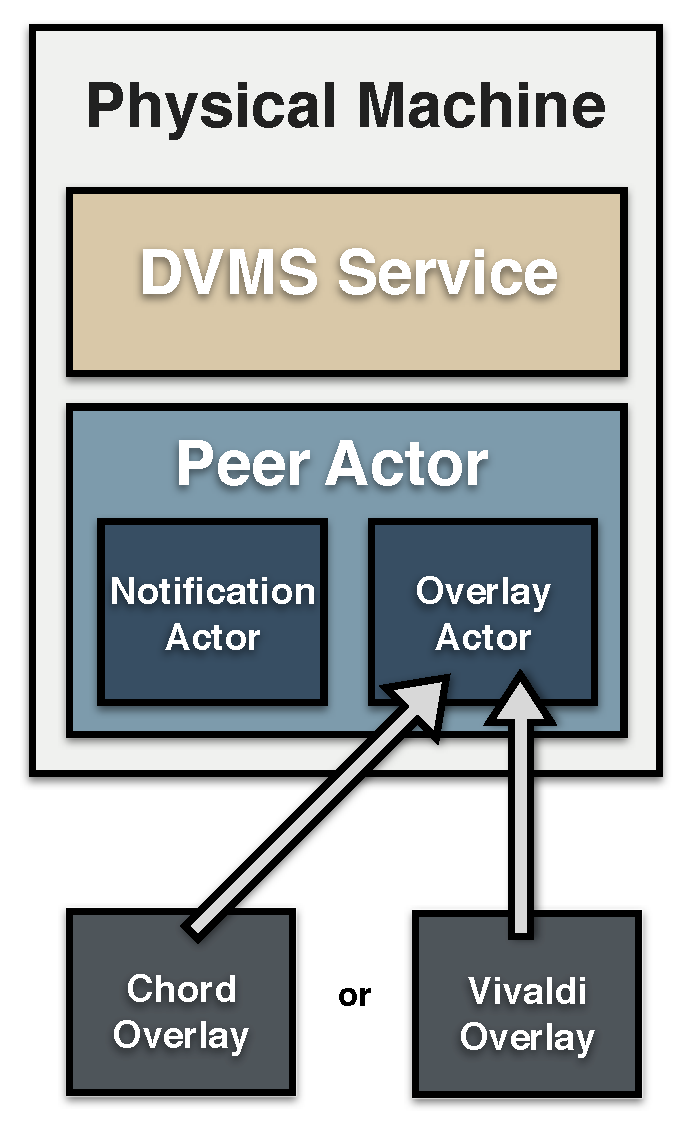
\includegraphics[width=\linewidth]{Figures/DVMS.pdf}
  \caption{DVMS on top of the Peer actor.}%
  \label{fig:peeractor}%
%\end{figure}
\end{wrapfigure}

From the software point of view, the Peer actor relies on modern piece of
software (Scala and akka)  following  the actor model rules.  In such a model,
each instance will collaborate by exclusively exchanging messages and priority
will be given to collaboration between close instances.  Such a coding approach
enables to tackle several issues of distributed systems such as deadlocks and
race conditions.


%%\subsubsection{Peer actor abstraction}
%
%%   * Peer actor:
%%		- apporte la tolerance aux pannes, abstraction du réseau, communication
%%		  interservices.
%%		- propose une API pour développer vite.
%At coarse-grained, the \emph{Peer actor} provides several features: fault tolerance,
%network abstraction and communication between services.
%%   * Peer actor deux sous acteurs:
%%		- notification actor: systeme a evenement pour les services.
%%		- network overlay actor: réseau avec implémentation chord et vivaldi.

As illustrated on Figure \ref {fig:peeractor}, the Peer actor contains two sub
actors: the \emph{Notification actor} and the \emph{Network overlay actor}. The
Notification actor enables services to subscribe to events that will be
triggered by other services. The Network overlay actor is in charge of
sending/receiving message through network. In order to compare both approaches, ring-based \vs locality-aware, we developed two different
network overlay actors: the first one provides a Chord-like overlay 
\cite{stoica2001chord}, while the second one delivers the locality-aware overlay described in Sec. \ref{ssec:lao}.

